\documentclass[11pt,a4paper]{article}

% ---------- Font ----------
\usepackage{newtxtext}
\usepackage{newtxmath}          % amssymb-এর বদলে; \Bbbk conflict এড়াতে

% ---------- Color ----------
\usepackage{xcolor}

% ---------- Geometry ----------
\usepackage{geometry}
\geometry{margin=1in}
\setlength{\emergencystretch}{3em} % Overfull hbox ঠিক করার জন্য

% ---------- Math & graphics ----------
\usepackage{amsmath}
\usepackage{graphicx}
\usepackage{booktabs}
\usepackage{array}
\usepackage{subcaption}
\usepackage{listings}
\usepackage{underscore}

% ---------- Section styling ----------
\usepackage{titlesec}
\titleformat{\section}
  {\normalfont\Large\bfseries\color{blue}}
  {\thesection}{1em}{}
\titleformat{\subsection}
  {\normalfont\large\bfseries\color{blue}}
  {\thesubsection}{1em}{}
\titleformat{\subsubsection}
  {\normalfont\normalsize\bfseries\color{blue}}
  {\thesubsubsection}{1em}{}
\titlespacing*{\section}{0pt}{12pt}{6pt}
\titlespacing*{\subsection}{0pt}{10pt}{4pt}

% ---------- Bibliography (biblatex) ----------
\usepackage[style=numeric,backend=biber,sorting=none]{biblatex}
\addbibresource{references.bib}

% Bold author names in references
\renewcommand*{\mkbibnamefamily}[1]{\textbf{#1}}
\renewcommand*{\mkbibnamegiven}[1]{\textbf{#1}}

% ---------- Hyperref (সবার শেষে) ----------
% xurl প্যাকেজ লম্বা লিংক ভাঙার জন্য
\usepackage{xurl} 
\usepackage[colorlinks=true,
            linkcolor=blue,
            citecolor=blue,
            urlcolor=blue,
            filecolor=blue]{hyperref}

% DOI-এর ডুপ্লিকেট টেক্সট বাদ দেওয়া এবং লিংক ভাঙার জন্য
\usepackage{doi}
\renewcommand{\doitext}{DOI: } 

% ---------- TikZ ----------
\usepackage{tikz}
\usetikzlibrary{arrows.meta,positioning,fit,backgrounds,calc,shapes.geometric}

% ---------- Custom macros ----------
\newcommand{\XT}{\textsc{XThreat}}
\newcommand{\feat}[1]{\texttt{#1}}

% ---------- Listing style ----------
\lstset{
  basicstyle=\ttfamily\footnotesize,
  breaklines=true,
  frame=single,
  columns=fullflexible,
  keepspaces=true,
  showstringspaces=false
}

% ---------- Title info ----------
\title{\textbf{XThreat: Explainable and Evidence-Aware AI\\for Cyber Threat Detection}}
\author{Ashabul Yamin Tuhin\\
Department of Computer Science and Engineering\\
International Islamic University Chittagong (IIUC), Chattogram, Bangladesh}

\begin{document}
\maketitle

\begin{abstract}
A network-intrusion alert that says only ``attack detected'' gives a security analyst no basis for trusting, triaging or acting on it. This paper presents \XT, a pipeline that turns a flow-level prediction into a structured analyst report: \emph{attack detected $\rightarrow$ why $\rightarrow$ evidence $\rightarrow$ important features $\rightarrow$ attack behaviour $\rightarrow$ confidence $\rightarrow$ recommended response}, and, unlike most explainable-IDS work, tests both the explanations and the claims made about the model. We train XGBoost and LightGBM (with Random Forest, Logistic Regression and an FT-style Transformer as comparators) on CIC-IDS2017 (2.83\,M flows, 15 classes) under a leakage-aware protocol, and explain alerts with SHAP, LIME, Integrated Gradients and a constrained counterfactual search that feed a rule-based evidence layer. XGBoost reaches 99.82\,\% accuracy and a macro-F1 of 0.834 (95\,\% paired-bootstrap interval 0.785--0.887) on 495{,}192 held-out flows; benign-versus-attack F1 is 0.996 with a 0.15\,\% false-alarm rate. A statistical validation layer yields six findings: (i) LightGBM and Random Forest are not significantly different from XGBoost, whereas the Transformer is clearly worse ($-0.153$ macro-F1); (ii) 51--74\,\% of random-split test flows have a near-identical training flow, and a per-class chronological split lowers macro-F1 to 0.723; (iii) SHAP and LIME share 27\,\% of their top-5 features against a chance level of 17\,\% (51\,\% against 23\,\% once correlated features are merged), and SHAP is the more faithful under deletion (AOPC 0.81 versus 0.59); (iv) attribution does not imply necessity: SHAP gives the destination port the largest weight for FTP- and SSH-Patator, yet removing the port leaves detection intact; (v) the probabilities are already well calibrated (ECE 0.0005) and split-conformal sets flag 0.12\,\% of flows as ambiguous, while marginal coverage hides class-level failures (Brute Force 0.59, 0.99 with class-conditional sets); and (vi) a constrained counterfactual search changes 2 features instead of 10, never edits the port, and yields plausible counterfactuals for 27\,\% of alerts against none for the greedy search. Graph neural networks and cross-dataset testing remain future work.
\end{abstract}

\noindent\textbf{Keywords:} intrusion detection, explainable AI, SHAP, LIME, counterfactual explanation, calibration, conformal prediction, CIC-IDS2017, analyst trust.

% =====================================================================
\section{Introduction}
\label{sec:intro}

Flow-level classifiers trained on benchmarks such as CIC-IDS2017 \parencite{sharafaldin2018} routinely exceed 99\,\% accuracy, and gradient-boosted trees are among the strongest and cheapest models for such tabular data \parencite{chen2016,ke2017,grinsztajn2022}. In a Security Operations Centre (SOC), however, an alert is useful only if the analyst can decide whether to believe it, how to prioritise it and what to do next \parencite{doshivelez2017,lipton2018,miller2019}; interviews with SOC analysts report that contextual, evidence-backed explanations matter more to them than raw outputs \parencite{eriksson2022,rastogi2025}.

Explainable-AI (XAI) methods supply the building blocks - Shapley attributions \parencite{lundberg2017,lundberg2020}, local surrogates \parencite{ribeiro2016} and counterfactuals \parencite{wachter2018} - and many studies apply them to intrusion detection \parencite{wang2020,mane2021,neupane2022}. Three gaps remain. First, most work stops at a feature-importance plot rather than an \emph{evidence chain} that an analyst can read. Second, the explanations are seldom tested: different explainers often disagree \parencite{krishna2024,dietz2024,kumar2025}, and a model can attribute its decision to a feature it does not need or to a dataset artefact. Third, the claims made about the detector itself are rarely backed by uncertainty estimates: a single split, a single seed and an uncalibrated ``confidence'' make it impossible to say whether a difference between two models, or a reported probability, can be trusted. This paper addresses these gaps with \XT{}, structured around four research questions:
\begin{itemize}
  \item \textbf{RQ1} How well do tree ensembles detect and classify CIC-IDS2017 flows under a leakage-aware protocol, and how much does the result depend on the evaluation split?
  \item \textbf{RQ2} Can SHAP, LIME and counterfactual outputs be converted into a traceable, seven-stage analyst report?
  \item \textbf{RQ3} How reliable are the explanations: do SHAP and LIME agree beyond chance, which of them is more faithful, does attribution imply necessity, and can explanations expose dataset shortcuts?
  \item \textbf{RQ4} Does the ``confidence'' stage deserve trust: are the probabilities calibrated, and can conformal prediction sets tell the analyst which alerts to double-check?
\end{itemize}

\paragraph{Contributions.} (1) A leakage-aware CIC-IDS2017 pipeline with row accounting at every step and a capped resampling policy that avoids oversampling classes with fewer than 50 real samples (Section~\ref{sec:data}). (2) A per-class chronological split that keeps all 15 classes in both partitions, a near-duplicate audit with a group-aware split, and paired bootstrap, multi-seed and significance analyses that include a Transformer comparator (Sections~\ref{sec:validation} and \ref{sec:results}). (3) A rule-based evidence layer that turns SHAP attributions into the report required by the project brief, now with calibrated confidence and conformal prediction sets in the confidence stage (Sections~\ref{sec:method} and \ref{sec:results}). (4) A quantitative explanation audit---SHAP--LIME agreement against chance, cluster-level agreement, deletion fidelity, stability, a port ablation separating attribution from necessity and a documented shortcut case---together with constrained counterfactuals (Sections~\ref{sec:results} and \ref{sec:discussion}). (5) A comparison with recent literature.

% =====================================================================
\section{Related Work}
\label{sec:related}

\paragraph{Learning-based intrusion detection and dataset quality.} Surveys document the move from rule- and anomaly-based detection to supervised and deep models \parencite{buczak2016,vinayakumar2019}, while \textcite{sommer2010} and \textcite{arp2022} warn that security machine learning is prone to sampling bias, data snooping and spurious correlations. CIC-IDS2017 \parencite{sharafaldin2018} is widely used \parencite{panigrahi2018,maseer2021,ring2019}, but audits found flow-construction and labelling errors that change measured performance \parencite{engelen2021,lanvin2023}. Evaluation protocol matters as well: \textcite{moczkodan2026} rebuild CIC-IDS2017 as temporal sequences and report that padding convention and split protocol affect results more than architecture, that a plain time-based split is degenerate (only two of 13 classes reach the test set) and that a Transformer drops from 0.775 to 0.549 macro-F1 under a leakage-free group split while Random Forest stays at 0.778. Such results agree with the general finding that tree ensembles remain competitive on tabular data \parencite{grinsztajn2022,shwartzziv2022}, whereas graph models need addressing information \parencite{kipf2017,hamilton2017,lo2022}.

\paragraph{Explanation methods.} SHAP assigns Shapley values with axiomatic guarantees \parencite{lundberg2017}, computed exactly for trees by TreeSHAP \parencite{lundberg2020}; LIME fits a local sparse linear surrogate \parencite{ribeiro2016}; counterfactual explanations ask what would have to change to alter the decision \parencite{wachter2018,mothilal2020}. All have known weaknesses: manipulability \parencite{slack2020}, instability \parencite{alvarezmelis2018} and, above all, mutual \emph{disagreement}, which practitioners resolve with ad-hoc heuristics \parencite{krishna2024}.

\paragraph{Explainable and evaluated intrusion detection.} Table~\ref{tab:related} summarises recent work closest to ours. Earlier studies mostly present feature-importance plots \parencite{marino2018,wang2020,mane2021,neupane2022}; \textcite{warnecke2020} showed that explanation methods differ substantially in fidelity for security models. Recent studies begin to evaluate explanations, but each isolates one aspect (agreement, faithfulness, counterfactual quality or user needs), usually on a different dataset or model family. To our knowledge, none of these studies combines, on the same alerts, an agreement audit with chance baselines, a fidelity test, a necessity test, calibrated uncertainty and a shortcut check with a generated analyst report, which is the niche of \XT.

\paragraph{Uncertainty, calibration and statistical comparison.} Accuracy and a single macro-F1 value do not say how far a reported probability can be trusted. Modern classifiers can be miscalibrated, and temperature scaling is a simple post-hoc remedy \parencite{guo2017}. Conformal prediction \parencite{vovk2005,angelopoulos2023} goes further: with a held-out calibration set it returns a \emph{set} of labels whose marginal coverage is guaranteed under exchangeability, and class-conditional (Mondrian) variants give per-class coverage when enough calibration data exist. Differences between models on one test set should be accompanied by bootstrap intervals \parencite{efron1993}, paired tests such as McNemar's \parencite{mcnemar1947} and a metric that stays informative under imbalance, such as the Matthews correlation coefficient \parencite{matthews1975}. For explanations, Integrated Gradients \parencite{sundararajan2017} gives attributions with a completeness property for differentiable models, and deletion-based curves \parencite{samek2017} measure whether the highest-ranked features really change the output.

\begin{table}[tbp]
\centering
\caption{Recent related studies (2022--2026) compared with this work.}
\label{tab:related}
\scriptsize
\renewcommand{\arraystretch}{1.12}
\resizebox{\textwidth}{!}{%
\begin{tabular}{>{\raggedright\arraybackslash}p{2.6cm}>{\raggedright\arraybackslash}p{3.0cm}>{\raggedright\arraybackslash}p{3.2cm}>{\raggedright\arraybackslash}p{6.4cm}}
\toprule
Study & Data / models & Explanation focus & Reported finding\\
\midrule
\textcite{srisumrith2026} & CIC-IDS2017 (20\,\% sample); XGBoost, RF, LR & SHAP (on RF); leakage screening of 29 of 78 features & Macro-F1 up to 0.997 under random splits; no evaluation of the explanations\\
\textcite{moczkodan2026} & CIC-IDS2017 sequences; 9 models & None (split and padding protocol) & Random vs.\ group split changes ranking; time split degenerate; RF most robust (0.778)\\
\textcite{dietz2024} & Several NIDS datasets and models & SHAP, LIME, TreeInterpreter, Saliency, IG, DeepLIFT & Consensus between methods varies from high to low\\
\textcite{kumar2025} & Kitsune, HorusEye, ENIDrift, HELAD; Mirai, CIC-IDS2017 & TRUSTEE vs.\ SHAP & Agreement between 0.0 and 0.38 depending on the model\\
\textcite{hermosilla2025} & UNSW-NB15; XGBoost, TabNet & SHAP and LIME (forensics) & Methods complementary; XGBoost explanations more stable than TabNet (Jaccard 0.82 vs.\ 0.65)\\
\textcite{kalakoti2025} & Real SOC Suricata alerts; LSTM & LIME, SHAP, IG, DeepLIFT & Faithfulness correlation: SHAP 0.40, LIME 0.42, DeepLIFT 0.76\\
\textcite{galwaduge2025} & UNSW-NB15, CIC-DDoS-2019, CIC-IDS2017; binary & Diffusion-based counterfactuals & High validity and plausibility; unconstrained baselines perform poorly\\
\textcite{eriksson2022,rastogi2025} & SOC analyst interviews (and 248-person survey) & SHAP/LIME alerts; explanation needs & Analysts value contextual, role-aware explanations\\
\midrule
\textbf{This work} & CIC-IDS2017, 15 classes; XGBoost, LightGBM, RF, LR, FT-Transformer & SHAP, LIME, IG, constrained counterfactual + evidence layer & Agreement vs.\ chance, AOPC fidelity, port ablation, shortcut case, conformal sets, chronological split, paired bootstrap\\
\bottomrule
\end{tabular}}
\end{table}

% =====================================================================
\section{Methodology}
\label{sec:method}

\subsection{Pipeline overview}
Figure~\ref{fig:pipeline} summarises the updated \XT{} pipeline. The \emph{detection half} (parts A and B: data to prediction) and the \emph{explanation half} (parts C and D: prediction to analyst report) are the pipeline prescribed by the project brief and share the same trained model and feature space, so every explanation refers to exactly the features the model used. The update adds a \emph{validation layer} (part E) that tests every stage statistically, and changes five components: the splitting step (A), the model set (B), the explainers (C), the confidence stage (D) and the counterfactual search (C). Violet boxes in Figure~\ref{fig:pipeline} mark what is new or changed; blue, green, orange and red boxes are unchanged.

\begin{figure}[tbp]
\centering
\resizebox{\textwidth}{!}{%
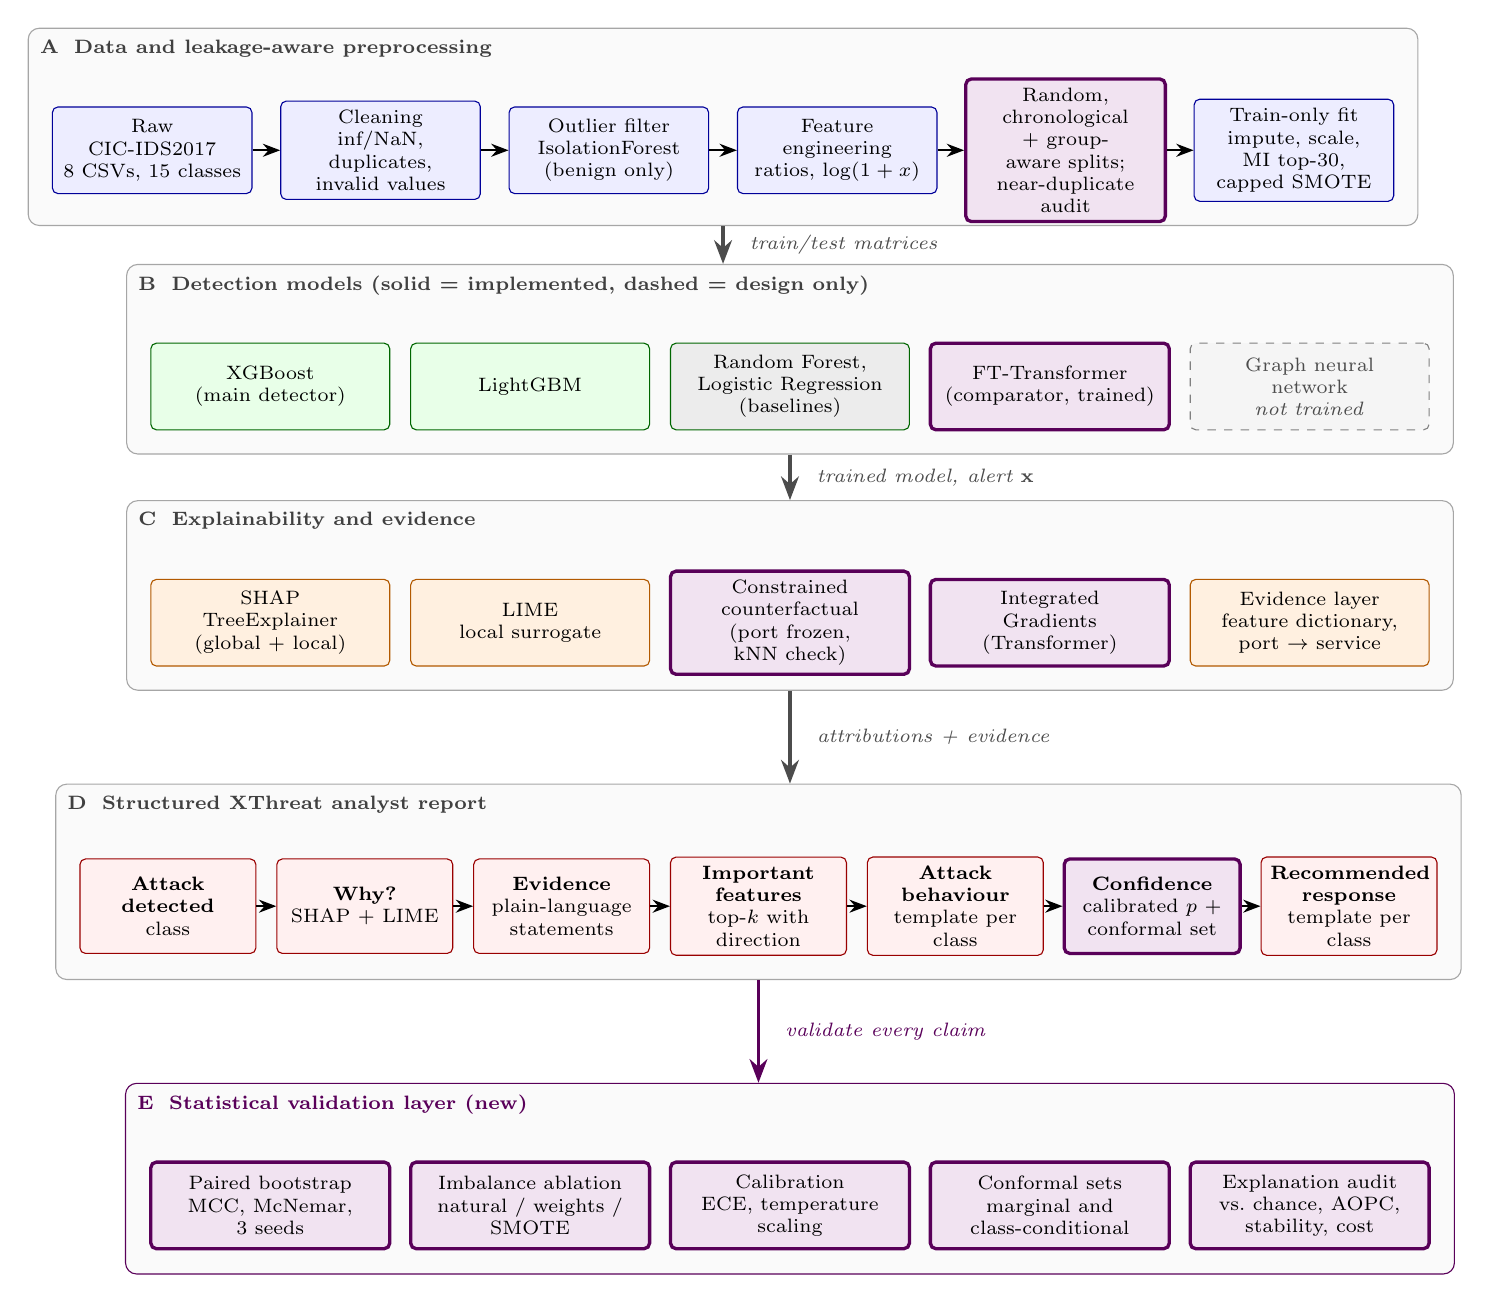
\begin{tikzpicture}[
  font=\scriptsize,
  box/.style={draw=blue!60!black, rounded corners=2pt, align=center, minimum height=11mm, text width=23mm, fill=blue!7},
  mbox/.style={draw=green!40!black, rounded corners=2pt, align=center, minimum height=11mm, text width=28mm, fill=green!9},
  nbox/.style={draw=gray, dashed, rounded corners=2pt, align=center, minimum height=11mm, text width=28mm, fill=gray!8, text=gray!60!black},
  ebox/.style={draw=orange!70!black, rounded corners=2pt, align=center, minimum height=11mm, text width=28mm, fill=orange!12},
  rbox/.style={draw=red!60!black, rounded corners=2pt, align=center, minimum height=12mm, text width=20mm, fill=red!6},
  vbox/.style={draw=violet!70!black, very thick, rounded corners=2pt, align=center, minimum height=11mm, text width=28mm, fill=violet!11},
  grp/.style={draw=black!35, rounded corners=4pt, inner sep=3mm, fill=black!2},
  glab/.style={font=\scriptsize\bfseries, text=black!75, anchor=north west, inner sep=1.5mm},
  arr/.style={-{Stealth[length=2.2mm]}, thick},
  garr/.style={-{Stealth[length=3mm]}, line width=1.4pt, black!70}
]
% ---- A: data and preprocessing
\node[box] (a1) at (0,0) {Raw\\CIC-IDS2017\\8 CSVs, 15 classes};
\node[box] (a2) at (2.9,0) {Cleaning\\inf/NaN, duplicates,\\invalid values};
\node[box] (a3) at (5.8,0) {Outlier filter\\IsolationForest\\(benign only)};
\node[box] (a4) at (8.7,0) {Feature\\engineering\\ratios, $\log(1+x)$};
\node[vbox, text width=23mm] (a5) at (11.6,0) {Random, chronological\\+ group-aware splits;\\near-duplicate audit};
\node[box] (a6) at (14.5,0) {Train-only fit\\impute, scale, MI top-30, capped SMOTE};
\draw[arr] (a1)--(a2); \draw[arr] (a2)--(a3); \draw[arr] (a3)--(a4); \draw[arr] (a4)--(a5); \draw[arr] (a5)--(a6);
\coordinate (GAp) at (7.3,1.25);
\begin{scope}[on background layer]
\node[grp, fit=(a1)(a6)(GAp)] (GA) {};
\end{scope}
\node[glab] at (GA.north west) {A\; Data and leakage-aware preprocessing};
% ---- B: models
\node[mbox] (b1) at (1.5,-3.0) {XGBoost\\(main detector)};
\node[mbox] (b2) at (4.8,-3.0) {LightGBM};
\node[mbox, fill=gray!15] (b3) at (8.1,-3.0) {Random Forest,\\Logistic Regression\\(baselines)};
\node[vbox] (b4) at (11.4,-3.0) {FT-Transformer\\(comparator, trained)};
\node[nbox] (b5) at (14.7,-3.0) {Graph neural\\network\\\emph{not trained}};
\coordinate (GBp) at (7.3,-1.75);
\begin{scope}[on background layer]
\node[grp, fit=(b1)(b5)(GBp)] (GB) {};
\end{scope}
\node[glab] at (GB.north west) {B\; Detection models (solid = implemented, dashed = design only)};
% ---- C: explainability
\node[ebox] (c1) at (1.5,-6.0) {SHAP\\TreeExplainer\\(global + local)};
\node[ebox] (c2) at (4.8,-6.0) {LIME\\local surrogate};
\node[vbox] (c3) at (8.1,-6.0) {Constrained\\counterfactual\\(port frozen, kNN check)};
\node[vbox] (c4) at (11.4,-6.0) {Integrated\\Gradients\\(Transformer)};
\node[ebox] (c5) at (14.7,-6.0) {Evidence layer\\feature dictionary,\\port $\to$ service};
\coordinate (GCp) at (7.3,-4.75);
\begin{scope}[on background layer]
\node[grp, fit=(c1)(c5)(GCp)] (GC) {};
\end{scope}
\node[glab] at (GC.north west) {C\; Explainability and evidence};
% ---- D: report
\node[rbox] (d1) at (0.2,-9.6) {\textbf{Attack detected}\\class};
\node[rbox] (d2) at (2.7,-9.6) {\textbf{Why?}\\SHAP + LIME};
\node[rbox] (d3) at (5.2,-9.6) {\textbf{Evidence}\\plain-language\\statements};
\node[rbox] (d4) at (7.7,-9.6) {\textbf{Important features}\\top-$k$ with\\direction};
\node[rbox] (d5) at (10.2,-9.6) {\textbf{Attack behaviour}\\template per\\class};
\node[rbox, draw=violet!70!black, very thick, fill=violet!11] (d6) at (12.7,-9.6) {\textbf{Confidence}\\calibrated $p$ +\\conformal set};
\node[rbox] (d7) at (15.2,-9.6) {\textbf{Recommended response}\\template per\\class};
\foreach \i/\j in {d1/d2,d2/d3,d3/d4,d4/d5,d5/d6,d6/d7} \draw[arr] (\i)--(\j);
\coordinate (GDp) at (7.3,-8.35);
\begin{scope}[on background layer]
\node[grp, fit=(d1)(d7)(GDp)] (GD) {};
\end{scope}
\node[glab] at (GD.north west) {D\; Structured XThreat analyst report};
% ---- E: validation layer (new)
\node[vbox] (e1) at (1.5,-13.4) {Paired bootstrap\\MCC, McNemar,\\3 seeds};
\node[vbox] (e2) at (4.8,-13.4) {Imbalance ablation\\natural / weights /\\SMOTE};
\node[vbox] (e3) at (8.1,-13.4) {Calibration\\ECE, temperature\\scaling};
\node[vbox] (e4) at (11.4,-13.4) {Conformal sets\\marginal and\\class-conditional};
\node[vbox] (e5) at (14.7,-13.4) {Explanation audit\\vs.\ chance, AOPC,\\stability, cost};
\coordinate (GEp) at (7.3,-12.15);
\begin{scope}[on background layer]
\node[grp, draw=violet!70!black, fit=(e1)(e5)(GEp)] (GE) {};
\end{scope}
\node[glab, text=violet!70!black] at (GE.north west) {E\; Statistical validation layer (new)};
% ---- between groups
\draw[garr] (GA.south) -- node[right=2mm, font=\scriptsize\itshape]{train/test matrices} (GB.north -| GA.south);
\draw[garr] (GB.south) -- node[right=2mm, font=\scriptsize\itshape]{trained model, alert $\mathbf{x}$} (GC.north -| GB.south);
\draw[garr] (GC.south) -- node[right=2mm, font=\scriptsize\itshape]{attributions + evidence} (GD.north -| GC.south);
\draw[garr, violet!70!black] (GD.south) -- node[right=2mm, font=\scriptsize\itshape]{validate every claim} (GE.north -| GD.south);
\end{tikzpicture}}
\caption{The updated \XT{} pipeline. (A) Leakage-aware data preparation, now with a group-aware split and a near-duplicate audit; (B) detection models, where XGBoost and LightGBM are the main detectors, Random Forest and Logistic Regression are baselines, an FT-style Transformer is trained as a comparator and the graph neural network (dashed) remains design-only; (C) explanation components feeding the evidence layer, with a constrained counterfactual search and Integrated Gradients added; (D) the structured analyst report, which follows the sequence required by the project brief (attack detected $\rightarrow$ why $\rightarrow$ evidence $\rightarrow$ important features $\rightarrow$ attack behaviour $\rightarrow$ confidence $\rightarrow$ recommended response), with a calibrated, set-valued confidence stage; (E) the statistical validation layer. Violet boxes are new or changed relative to the pipeline prescribed by the project brief.}
\label{fig:pipeline}
\end{figure}

\subsection{Problem formulation and protocol}
Let $\mathcal{D}=\{(\mathbf{x}_i,y_i)\}_{i=1}^{N}$ be flow records with $\mathbf{x}_i\in\mathbb{R}^{d}$ and $y_i\in\{1,\dots,K\}$, $K=15$. The detector $f_\theta:\mathbb{R}^{d}\to\Delta^{K-1}$ returns class probabilities $p_k(\mathbf{x})$, the decision is $\hat{y}=\arg\max_k p_k(\mathbf{x})$ and the raw confidence is $c=\max_k p_k(\mathbf{x})$. In the updated pipeline the confidence stage reports a temperature-scaled $c$ together with a conformal prediction set $\mathcal{C}_\alpha(\mathbf{x})\subseteq\{1,\dots,K\}$. For each alert ($\hat{y}\neq\text{BENIGN}$) the system outputs $\mathcal{E}(\mathbf{x})=(\text{why},\text{evidence},\text{top features},\text{behaviour},c,\mathcal{C}_\alpha,\text{response})$.

\paragraph{Leakage-prevention rules.} Every statistic that depends on the data distribution (imputer medians, scaler parameters, mutual-information ranking, SMOTE neighbours) is estimated on the training partition only. Row-wise, parameter-free transformations ($\log(1+x)$, ratios) are applied before the split. The test set is never resampled. Variables that encode provenance rather than flow behaviour (the day or file a flow came from) are excluded, because they do not exist at deployment time.

\paragraph{Evaluation protocol.} Detection is evaluated on (a) a stratified 80/20 random split (the main results), (b) a per-class chronological split and (c) a group-aware split that keeps near-duplicate flows together (Sections~\ref{sec:data} and \ref{sec:validation}). Uncertainty is reported by a bootstrap over the test confusion matrix, by a paired bootstrap over test rows, by 5-fold cross-validation on the training partition and by three further seeds. Explanations are evaluated on random-split test flows only (Section~\ref{sec:metrics}).

\subsection{Detection layer}
XGBoost fits an additive tree ensemble $F(\mathbf{x})=\sum_t\eta\,h_t(\mathbf{x})$ by minimising a regularised loss, with softmax outputs and per-sample weights $w_i$ \parencite{chen2016}; LightGBM uses histogram-based, leaf-wise growth with early stopping \parencite{ke2017}. A Random Forest and a multinomial Logistic Regression serve as baselines to show how much of the performance comes from the data rather than from boosting. In the updated pipeline an FT-Transformer-style model \parencite{gorishniy2021} embeds each of the 30 selected features as a token, applies self-attention \parencite{vaswani2017} and classifies from a class token; it tests whether a deep tabular model can replace the tree ensembles \parencite{grinsztajn2022,shwartzziv2022}.

\subsection{Explanation layer}
\paragraph{SHAP.} The Shapley value of feature $j$ is $\phi_j(\mathbf{x})=\sum_{S\subseteq F\setminus\{j\}}\frac{|S|!\,(|F|-|S|-1)!}{|F|!}[f_{S\cup\{j\}}(\mathbf{x})-f_S(\mathbf{x})]$, giving the additive explanation $f(\mathbf{x})=\phi_0+\sum_j\phi_j(\mathbf{x})$ \parencite{lundberg2017}; TreeSHAP computes it exactly for trees \parencite{lundberg2020}. For the multiclass model the values are in log-odds, one set per class; global importance is $\frac1n\sum_i|\phi_j(\mathbf{x}_i)|$.

\paragraph{LIME.} LIME samples perturbations around $\mathbf{x}$ and fits a weighted sparse linear surrogate, $\xi(\mathbf{x})=\arg\min_{g\in G}\mathcal{L}(f,g,\pi_{\mathbf{x}})+\Omega(g)$ \parencite{ribeiro2016}; weights are in probability units and tabular features are quantile-binned, which yields interval rules.

\paragraph{Integrated Gradients.} For the Transformer, the attribution of feature $j$ is $\mathrm{IG}_j(\mathbf{x})=(x_j-x'_j)\int_0^1\partial f(\mathbf{x}'+\lambda(\mathbf{x}-\mathbf{x}'))/\partial x_j\,d\lambda$ with the mean benign flow as baseline $\mathbf{x}'$ \parencite{sundararajan2017}; completeness requires $\sum_j\mathrm{IG}_j=f(\mathbf{x})-f(\mathbf{x}')$, which is checked numerically.

\paragraph{Counterfactual search.} Following \textcite{wachter2018}, a counterfactual $\mathbf{x}'$ is a nearby instance assigned to a target class $t$ (BENIGN). The \emph{greedy baseline} is transparent and library-free: with $\boldsymbol{\mu}_t$ the mean training vector of class $t$, each iteration moves the $k=10$ features with the largest gap $|\mu_{t,j}-x_j|$ a fraction $\alpha=0.2$ towards $\boldsymbol{\mu}_t$, $x_j\leftarrow x_j+\alpha(\mu_{t,j}-x_j)$, until the arg-max flips or an iteration limit is reached; it has no plausibility or actionability constraint (cf.\ \citeauthor{galwaduge2025}). The \emph{constrained search} of the updated pipeline (i) freezes \feat{Destination Port}, (ii) clips every feature to the 1--99\,\% range of benign training flows, (iii) prunes the change set to the smallest subset that still flips the prediction and (iv) checks plausibility by the $k$-nearest-neighbour distance to benign training flows against a benign-neighbourhood threshold.

\subsection{Evidence layer}
The evidence layer is a deterministic mapping from model output to analyst language with three parts: (i) a dictionary from feature names to plain meanings (e.g.\ \feat{Init_Win_bytes_backward} $\mapsto$ ``initial TCP window size, server side''); (ii) templates that produce ``abnormally high/low \emph{meaning}'' from the SHAP sign and the position of the instance relative to the mean benign flow, and that describe the destination port as a service (``targets port 21 (FTP)'') from the un-scaled port; and (iii) per-class dictionaries of attack-behaviour narratives and recommended responses for all 15 classes. Rule-based generation was chosen deliberately: every sentence is traceable to a feature, a SHAP value or a template, so the report cannot hallucinate.

\subsection{Validation layer}
\label{sec:validation}
\paragraph{Uncertainty and significance.} A paired bootstrap resamples the same 1{,}000 sets of test rows for two models and gives a confidence interval for the macro-F1 difference \parencite{efron1993}; McNemar's test \parencite{mcnemar1947}, the multiclass Matthews correlation coefficient \parencite{matthews1975} and balanced accuracy complement accuracy. Three further seeds (11, 22, 33) re-draw the split, the resampling, the feature selection and the model initialisation.

\paragraph{Near-duplicates and imbalance.} A test flow is a \emph{near-duplicate} if its 30 selected log-scale features, rounded to one or to zero decimals, equal those of at least one training flow. A \texttt{GroupShuffleSplit} over these keys gives the group-aware split. The \emph{imbalance ablation} compares natural unweighted training, capped square-root inverse-frequency weights and capped SMOTE, with everything else fixed.

\paragraph{Calibration and conformal prediction.} Expected calibration error (ECE), Brier score and negative log-likelihood are computed for raw and temperature-scaled probabilities \parencite{guo2017}; the temperature is fitted on a class-stratified 30\,\% calibration part of the test flows and all calibration and conformal results are evaluated on the remaining 70\,\%. Split-conformal sets \parencite{vovk2005,angelopoulos2023} use the score $s(\mathbf{x},y)=1-p_y(\mathbf{x})$, the threshold $\hat q$ is the $\lceil(n+1)(1-\alpha)\rceil/n$ empirical quantile of the calibration scores with $\alpha=0.05$, and $\mathcal{C}_\alpha(\mathbf{x})=\{k: 1-p_k(\mathbf{x})\leq\hat q\}$. The class-conditional (Mondrian) variant computes one threshold per class and falls back to the marginal threshold for classes with fewer than 20 calibration flows.

\paragraph{Explanation audit.} On up to eight flows per predicted attack class (55 flows from 11 classes), SHAP and LIME rankings of the predicted class are compared by \emph{overlap@$k$} against its chance level $k/30$, Spearman correlation of the absolute attributions, sign agreement of shared features (chance 0.5) and \emph{cluster-level overlap}, which merges the 30 features into 13 clusters of mutually correlated features ($|r|>0.9$). \emph{Deletion fidelity} measures the area over the perturbation curve (AOPC) \parencite{samek2017} when the top-ranked features are replaced by their benign mean, together with the sufficiency of the top-5 features, against a random ranking. SHAP \emph{stability} is the Jaccard overlap of the top-5 features under Gaussian input noise ($\sigma=0.1$), and LIME \emph{self-consistency} is the overlap between two LIME runs with different seeds.

% =====================================================================
\section{Dataset and Preprocessing}
\label{sec:data}

\paragraph{Dataset.} CIC-IDS2017 \parencite{sharafaldin2018} (\texttt{MachineLearningCSV}) contains CICFlowMeter statistics for five days of testbed traffic in eight CSV files: 2{,}830{,}743 rows, 78 numeric features and a label. Attacks are scheduled by day (FTP/SSH-Patator on Tuesday; DoS and Heartbleed on Wednesday; web attacks and infiltration on Thursday; Bot, PortScan and DDoS on Friday). Benign traffic is 80.3\,\% of rows, while Heartbleed (11), Web Attack--SQL Injection (21) and Infiltration (36) are practically negligible (Table~\ref{tab:classes}). A \texttt{SourceDay} column added at loading is used only for bookkeeping and the chronological split.

\begin{table}[tbp]
\centering
\caption{Class distribution: raw, natural training split (80\,\%) and training set after capped resampling.}
\label{tab:classes}
\scriptsize
\resizebox{\textwidth}{!}{%
\begin{tabular}{lrrr@{\hspace{1.6em}}lrrr}
\toprule
Class & Raw & Train & Resampled & Class & Raw & Train & Resampled\\
\midrule
BENIGN & 2{,}273{,}097 & 1{,}640{,}229 & 1{,}640{,}229 & FTP-Patator & 7{,}938 & 4{,}743 & 10{,}000\\
DoS Hulk & 231{,}073 & 138{,}153 & 138{,}153 & SSH-Patator & 5{,}897 & 2{,}574 & 10{,}000\\
PortScan & 158{,}930 & 72{,}655 & 72{,}655 & DoS slowloris & 5{,}796 & 4{,}299 & 10{,}000\\
DDoS & 128{,}027 & 102{,}397 & 102{,}397 & DoS Slowhttptest & 5{,}499 & 4{,}182 & 10{,}000\\
DoS GoldenEye & 10{,}293 & 8{,}222 & 10{,}000 & Bot & 1{,}966 & 1{,}562 & 10{,}000\\
Web Att.\ -- Brute Force & 1{,}507 & 1{,}176 & 10{,}000 & Web Att.\ -- XSS & 652 & 522 & 10{,}000\\
Infiltration & 36 & 28 & 28 & Web Att.\ -- SQL Inj. & 21 & 17 & 17\\
Heartbleed & 11 & 6 & 6 & \textbf{Total} & \textbf{2{,}830{,}743} & \textbf{1{,}980{,}765} & \textbf{2{,}033{,}485}\\
\bottomrule
\end{tabular}}
\end{table}

\paragraph{Cleaning.} Initial inspection found 4{,}376 infinite values (in \feat{Flow Bytes/s} and \feat{Flow Packets/s} when duration is zero), 1{,}358 missing values, 331{,}200 duplicate rows, a duplicated column (\feat{Fwd Header Length.1}), negative values in time/rate columns and corrupted web-attack labels. Infinities were set to NaN and filled with the column median (0.1013\,\% of values; no column exceeded the 40\,\% deletion threshold); the duplicate column was dropped; labels were repaired to 15 consistent classes; 331{,}200 duplicate rows (11.70\,\%) and 2{,}881 flows with physically impossible negative time or rate values (0.115\,\%) were removed (Table~\ref{tab:prep}).

\paragraph{Outliers.} IQR and $|z|>3$ rules were used as diagnostics only, because extreme values are often the attack signal. The single outlier operation is an Isolation Forest \parencite{liu2008} fitted on benign flows only, removing the 1\,\% most isolated benign rows (20{,}705) as likely noise; attack rows are never removed.

\paragraph{Statistical analysis.} Welch's $t$, Mann--Whitney $U$ and Cohen's $d$ for key features showed that effect sizes, not $p$-values (numerically zero at this sample size), are informative: the largest are \feat{Bwd Packet Length Mean} ($d=1.31$), \feat{Flow Duration} ($0.70$) and \feat{Flow IAT Mean} ($0.54$). A one-way ANOVA of \feat{Flow Duration} across attack types ($F=55{,}640$) and a $\chi^2$ test of well-known-port targeting against the label ($\chi^2=3{,}379$) were also significant.

\begin{table}[tbp]
\centering
\caption{Preprocessing steps and resulting row counts.}
\label{tab:prep}
\scriptsize
\resizebox{\textwidth}{!}{%
\begin{tabular}{p{4.2cm}p{5.6cm}r}
\toprule
Step & Action & Rows after step\\
\midrule
Merge 8 CSV files & concatenate, cast to float32 & 2{,}830{,}743\\
Duplicate rows & remove 331{,}200 (11.70\,\%) & 2{,}499{,}543$^{\dagger}$\\
Invalid time/rate values & remove 2{,}881 (0.115\,\%) & 2{,}496{,}662\\
Isolation Forest on BENIGN & remove 20{,}705 (1.00\,\% of benign) & 2{,}475{,}957\\
Stratified 80/20 split & train / test & 1{,}980{,}765 / 495{,}192\\
Capped SMOTE (train only) & 8 classes raised to 10{,}000 & 2{,}033{,}485 (train)\\
\bottomrule
\end{tabular}}
\\[1pt]{\scriptsize $^{\dagger}$Derived: $2{,}830{,}743-331{,}200$.}
\end{table}

\paragraph{Feature engineering and transformation.} Five features were added: \feat{Fwd_Bwd_Pkt_Ratio}, \feat{Bytes_per_Packet}, \feat{Fwd_Bwd_Byte_Ratio} (with $+1$ in denominators), \feat{Flag_Sum} (sum of six TCP flag counts) and \feat{Is_WellKnown_Port} (port $\leq1023$), giving $d=82$ candidates. A file-of-origin code (\feat{Day_Index}) used in an earlier configuration was removed as a provenance shortcut (Section~\ref{sec:discussion}). Labels were integer-encoded; $\log(1+x)$ was applied to the 64 non-negative features with skewness above 2 (e.g.\ 364.3 for \feat{Total Length of Fwd Packets}).

\paragraph{Split, scaling and feature selection.} A stratified 80/20 split (seed 42) yields 1{,}980{,}765 training and 495{,}192 test flows. Median imputer and \texttt{StandardScaler} were fitted on the training part only, and the 30 features with the highest mutual information with the label \parencite{pedregosa2011} were retained (Figure~\ref{fig:shapglobal} and Table~\ref{tab:shapclass} show which matter most; \feat{Destination Port} is among them). Mutual information ranks features individually and does not remove redundancy, so strongly correlated selected features (e.g.\ \feat{Total Length of Bwd Packets} and \feat{Subflow Bwd Bytes}) can share SHAP credit, which matters for interpretation (Section~\ref{sec:discussion}).

\paragraph{Capped resampling.} Benign flows outnumber Heartbleed by about $2.7\times10^5$ in training. Oversampling all classes to the benign size with SMOTE \parencite{chawla2002,lemaitre2017}, as an earlier configuration did, would create over 1.6\,M synthetic samples from six real ones and a 24.6\,M-row training set. The final policy: (i) classes with at least 50 real training samples and fewer than 10{,}000 are raised to 10{,}000 with SMOTE ($k=5$), adding 52{,}720 synthetic rows; (ii) classes with fewer than 50 real samples (Heartbleed, Infiltration, SQL injection) receive no synthetic data but a sample weight of $\min(50,10{,}000/n)=50$; (iii) the four large classes are untouched. The target of 10{,}000 and the weight cap were fixed a priori and not tuned on test data. Section~\ref{sec:imb} compares this policy with natural and weight-only training.

\paragraph{Chronological split.} Within each class, flows are ordered by weekday and original row order; the first 80\,\% train and the last 20\,\% test (1{,}980{,}767 / 495{,}190 flows, all 15 classes in both). A ``train on Monday--Thursday, test on Friday'' design is impossible because PortScan, DDoS and Bot occur only on Friday. This split assumes that CSV row order approximates capture time (no timestamp column exists); all fitted components were re-fitted on the chronological training part.

% =====================================================================
\section{Model Implementation and Metrics}
\label{sec:impl}
\label{sec:metrics}

Experiments used Python with pandas, scikit-learn \parencite{pedregosa2011}, imbalanced-learn \parencite{lemaitre2017}, XGBoost, LightGBM, SHAP and LIME; the seed was 42 for the main results and 11, 22 and 33 for the multi-seed study. Table~\ref{tab:hyper} lists the hyperparameters. LightGBM used a 10\,\% stratified validation split of the resampled training set for early stopping (patience 30; best iteration 186, validation multi-logloss 0.0189). Random Forest (100 trees) and Logistic Regression (300 iterations) were trained with the same sample weights on a stratified subsample of 500{,}007 resampled rows to bound run time. SHAP values were computed with \texttt{TreeExplainer} for 2{,}000 random test flows (tensor $2000\times30\times15$); LIME used \texttt{LimeTabularExplainer} with 2{,}000 perturbations per flow (1{,}500 in the 55-flow audit); the FT-style Transformer was trained for 10 epochs on 400{,}000 resampled training rows without hyperparameter tuning; the counterfactual search used $k=10$, $\alpha=0.2$, feature ranking refreshed every 5 iterations and at most 60 iterations. Over-fitting was checked with the train--test gap on natural data, stratified 5-fold cross-validation and a learning curve over 10--100\,\% stratified training subsets.

\begin{table}[tbp]
\centering
\caption{Hyperparameters of the two detectors.}
\label{tab:hyper}
\scriptsize
\resizebox{\textwidth}{!}{%
\begin{tabular}{lcc}
\toprule
Parameter & XGBoost & LightGBM\\
\midrule
Trees & 300 & 500 (early stop at 186)\\
Tree complexity & max\_depth $=8$ & num\_leaves $=63$\\
Learning rate & 0.1 & 0.05\\
Row / column subsampling & 0.8 / 0.8 & 0.8 / 0.8\\
Regularisation & default & $\alpha=\lambda=0.1$, min\_child\_samples $=50$\\
Objective / method & multi:softprob, hist & multiclass, histogram\\
\bottomrule
\end{tabular}}
\end{table}

\paragraph{Metrics.} Because 82.8\,\% of test flows are benign, accuracy is uninformative; we report per-class precision, recall and F1 \parencite{sokolova2009}, \textbf{macro-F1} (unweighted mean over $K=15$ classes, the headline metric), macro one-vs-rest ROC-AUC, row-normalised confusion matrices and a binary benign-versus-attack view (precision, recall, F1, ROC-AUC, PR-AUC, false-alarm rate $FP/(FP+TN)$, miss rate $FN/(FN+TP)$ with attack score $1-p_{\text{BENIGN}}$). A 95\,\% bootstrap interval for accuracy and macro-F1 was obtained by resampling each true class of the test confusion matrix multinomially (1{,}000 replicates); it captures test-sampling variability only, not training variability. \textbf{Explanation audit metrics} compare the SHAP and LIME rankings of the predicted class on the same alert: \emph{overlap@5} (fraction of SHAP top-5 features also in the LIME top-5), \emph{sign agreement} (fraction of shared features with identical sign) and \emph{top-1 agreement}; counterfactuals are summarised by success rate, number of changed features, L1/L2 shift in standardised units, whether the port was changed and plausibility. The validation layer adds the Matthews correlation coefficient and balanced accuracy, ECE, Brier score and negative log-likelihood, and the conformal coverage and set size (Section~\ref{sec:validation}).

% =====================================================================
\section{Experimental Results}
\label{sec:results}

\subsection{Detection performance (RQ1)}
Table~\ref{tab:overall} compares the models on the 495{,}192 test flows. All tree models exceed 99.7\,\% accuracy, but macro-F1 is 0.78--0.83 because of a few difficult classes. XGBoost is best (0.834; 95\,\% multinomial-bootstrap interval 0.780--0.882, paired row-bootstrap interval 0.785--0.887; accuracy interval 0.9981--0.9983), followed by Random Forest (0.822) and LightGBM (0.782); Logistic Regression (0.561) fails on Bot and all web attacks, confirming that the problem is non-linear. The paired bootstrap (Table~\ref{tab:paired}, Figure~\ref{fig:models}) shows that the tree ensembles cannot be separated: LightGBM ($-0.047$, 95\,\% CI $-0.098$ to $+0.001$) and Random Forest ($-0.021$, CI $-0.076$ to $+0.030$) are not significantly different from XGBoost, whereas Logistic Regression ($-0.267$) and the FT-style Transformer ($-0.153$, CI $-0.215$ to $-0.099$) are clearly worse. McNemar's test flags even small accuracy differences as significant because of the sample size, so the macro-F1 interval is the more informative statistic. Macro one-vs-rest ROC-AUC of XGBoost is 0.9996.

\begin{table}[tbp]
\centering
\caption{Overall test performance (495{,}192 flows).}
\label{tab:overall}
\small
\resizebox{\textwidth}{!}{%
\begin{tabular}{lcccc}
\toprule
Model & Accuracy & Macro-P & Macro-R & Macro-F1\\
\midrule
XGBoost & 0.9982 & 0.8656 & 0.8632 & \textbf{0.8336}\\
LightGBM & 0.9980 & 0.7473 & 0.8482 & 0.7821\\
Random Forest (baseline) & 0.9981 & 0.8551 & 0.8197 & 0.8224\\
Logistic Regression (baseline) & 0.9824 & 0.5440 & 0.6304 & 0.5614\\
\bottomrule
\end{tabular}}
\end{table}

\begin{table}[tbp]
\centering
\caption{Paired bootstrap on the main split (1{,}000 replicates of the test rows). $\Delta$F1 is the macro-F1 difference to XGBoost with its paired 95\,\% interval; McNemar's $p$ refers to the accuracy difference. MCC is the multiclass Matthews correlation coefficient.}
\label{tab:paired}
\scriptsize
\resizebox{\textwidth}{!}{%
\begin{tabular}{lccccc}
\toprule
Model & Macro-F1 & 95\,\% CI & MCC & $\Delta$F1 vs.\ XGBoost (paired CI) & McNemar $p$\\
\midrule
XGBoost & 0.8336 & [0.785, 0.887] & 0.9942 & -- & --\\
LightGBM & 0.7821 & [0.759, 0.818] & 0.9933 & $-0.047$ [$-0.098$, $+0.001$] & $9.6\times10^{-9}$\\
Random Forest & 0.8224 & [0.777, 0.848] & 0.9936 & $-0.021$ [$-0.076$, $+0.030$] & $8.9\times10^{-3}$\\
Logistic Regression & 0.5614 & [0.548, 0.600] & 0.9420 & $-0.267$ [$-0.319$, $-0.217$] & $<10^{-300}$\\
FT-Transformer & 0.6697 & -- & 0.9750 & $-0.153$ [$-0.215$, $-0.099$] & --\\
\bottomrule
\end{tabular}}
\end{table}

\begin{figure}[tbp]
\centering
\includegraphics[width=\textwidth]{figs/fig_pub_B_model_comparison.png}
\caption{Model comparison with bootstrap intervals, paired differences to XGBoost and the Transformer comparator.}
\label{fig:models}
\end{figure}

\paragraph{Binary view.} Collapsing to benign versus attack, XGBoost detects 85{,}066 of 85{,}134 attack flows (miss rate 0.080\,\%) and flags 619 of 410{,}058 benign flows (false-alarm rate 0.151\,\%); precision is 0.9928, F1 0.9960, ROC-AUC 0.99997 and PR-AUC 0.99986. The gap between this near-perfect detector and the macro-F1 of 0.83 shows that the remaining difficulty is \emph{naming} the attack, not \emph{detecting} it.

\subsection{Per-class analysis}
Table~\ref{tab:perclass} and Figure~\ref{fig:cm} give per-class results. Nine of 15 XGBoost classes reach F1 $\geq0.95$. Macro-F1 over the 12 classes with at least 130 test flows is 0.892, and over the ten non-web classes among them 0.978, so the headline value is driven by three issues:
\begin{itemize}
  \item \textbf{Web-attack confusion.} Of 294 Brute-Force flows 112 are predicted as XSS, and of 130 XSS flows 53 as Brute Force (F1 0.591 and 0.340). Flow statistics contain no HTTP payload, so the two attacks are nearly indistinguishable at this level.
  \item \textbf{False alarms.} Of 619 benign flows misclassified, 178 become PortScan, 162 Bot, 131 XSS, 75 Brute Force and 64 DoS Hulk; this explains the low precision of Bot (0.697) and XSS (0.238).
  \item \textbf{Tiny classes.} Heartbleed (1 test flow), Infiltration (7) and SQL injection (4) give statistically meaningless metrics; LightGBM finds no SQL-injection flow and the Random Forest is better on Brute Force and XSS (F1 0.672, 0.434).
\end{itemize}

\begin{table}[tbp]
\centering
\caption{Per-class test results. XGBoost: precision (P), recall (R), F1; other models: F1. The last column is XGBoost F1 under the per-class chronological split.}
\label{tab:perclass}
\scriptsize
\setlength{\tabcolsep}{3.4pt}
\resizebox{\textwidth}{!}{%
\begin{tabular}{lrcccccccc}
\toprule
 & & \multicolumn{3}{c}{XGBoost} & LGBM & RF & LR & XGB\\
Class & Support & P & R & F1 & F1 & F1 & F1 & F1 (chrono)\\
\midrule
BENIGN & 410{,}058 & 0.9998 & 0.9985 & 0.9992 & 0.9990 & 0.9991 & 0.9898 & 0.9795\\
Bot & 391 & 0.6966 & 0.9514 & 0.8043 & 0.8068 & 0.8235 & 0.0000 & 0.1323\\
DDoS & 25{,}600 & 0.9998 & 0.9996 & 0.9997 & 0.9996 & 0.9996 & 0.9928 & 0.8346\\
DoS GoldenEye & 2{,}055 & 0.9966 & 0.9985 & 0.9976 & 0.9956 & 0.9932 & 0.8145 & 0.9698\\
DoS Hulk & 34{,}538 & 0.9978 & 0.9990 & 0.9984 & 0.9983 & 0.9970 & 0.9377 & 0.9683\\
DoS Slowhttptest & 1{,}046 & 0.9923 & 0.9904 & 0.9914 & 0.9914 & 0.9890 & 0.6884 & 0.8792\\
DoS slowloris & 1{,}075 & 0.9944 & 0.9926 & 0.9935 & 0.9944 & 0.9949 & 0.5634 & 0.8748\\
FTP-Patator & 1{,}186 & 1.0000 & 0.9992 & 0.9996 & 1.0000 & 0.9996 & 0.9408 & 0.9889\\
Heartbleed & 1 & 0.5000 & 1.0000 & 0.6667 & 0.6667 & 1.0000 & 0.5000 & 0.0000\\
Infiltration & 7 & 1.0000 & 0.5714 & 0.7273 & 0.4211 & 0.4444 & 0.1270 & 0.7143\\
PortScan & 18{,}164 & 0.9903 & 0.9996 & 0.9949 & 0.9949 & 0.9902 & 0.9781 & 0.9708\\
SSH-Patator & 643 & 1.0000 & 1.0000 & 1.0000 & 1.0000 & 1.0000 & 0.8891 & 0.9851\\
Web Att.\ -- Brute Force & 294 & 0.5779 & 0.6054 & 0.5914 & 0.5561 & 0.6716 & 0.0000 & 0.5359\\
Web Att.\ -- SQL Inj. & 4 & 1.0000 & 0.2500 & 0.4000 & 0.0000 & 0.0000 & 0.0000 & 0.7500\\
Web Att.\ -- XSS & 130 & 0.2384 & 0.5923 & 0.3400 & 0.3074 & 0.4342 & 0.0000 & 0.2652\\
\midrule
Macro-F1 & & & & 0.8336 & 0.7821 & 0.8224 & 0.5614 & 0.7232\\
\bottomrule
\end{tabular}}
\end{table}

\begin{figure}[tbp]
\centering
\includegraphics[width=0.66\textwidth]{figs/fig_confusion_matrix_xgb.png}
\caption{Row-normalised confusion matrix of XGBoost. Blank cells contain no flows; ``$<$.01'' marks non-zero cells below 0.005.}
\label{fig:cm}
\end{figure}

\subsection{Over-fitting and generalisation over time}
On the natural training split XGBoost reaches accuracy 0.9984 and macro-F1 0.9238, against 0.9982 and 0.8336 on the test set; the macro-F1 gap of 0.090 comes almost entirely from rare classes. Stratified 5-fold macro-F1 was 0.8764, 0.8981, 0.8456, 0.8681 and 0.8623 (mean 0.8701, SD 0.0173). The learning curve (Figure~\ref{fig:lc}) shows training macro-F1 falling from 0.958 to 0.923 and validation macro-F1 rising from 0.835 to 0.874 as training size grows from 168{,}380 to 1{,}683{,}650 flows, flat above about 0.8\,M flows: the bottleneck is the number of independent minority-class examples, not data volume.

Under the per-class chronological split (last column of Table~\ref{tab:perclass}), macro-F1 falls from 0.834 to 0.723 and accuracy from 0.9982 to 0.9635; benign recall drops to 0.9625, so 3.7\,\% of later benign flows are flagged, and Bot precision collapses to 0.071 and DDoS precision to 0.717. This is consistent with distribution shift within a day and with the finding that random splits overstate performance \parencite{moczkodan2026,arp2022}; unlike a Monday--Thursday/Friday split it keeps every class in both partitions. Classes with 1--7 test flows (Heartbleed, Infiltration, SQL injection) fluctuate arbitrarily and are not interpretable.

\begin{figure}[tbp]
\centering
\includegraphics[width=0.5\textwidth]{figs/fig_learning_curve.png}
\caption{Learning curve (macro-F1, stratified training subsets, fixed validation split).}
\label{fig:lc}
\end{figure}

\subsection{Seeds, near-duplicates and class imbalance (RQ1)}
\label{sec:imb}
\paragraph{Seeds.} Over seeds 11, 22 and 33 macro-F1 is $0.845\pm0.018$ for XGBoost (95\,\% $t$-interval half-width 0.045), $0.824\pm0.012$ for Random Forest and $0.810\pm0.016$ for LightGBM; the ranking changes with the seed (in seed 22 LightGBM leads), consistent with the paired bootstrap. Per-class standard deviations are near zero for large classes and large for Infiltration ($0.56\pm0.28$). Mutual-information selection was perfectly stable: the same 30 features were chosen in every seed (mean pairwise Jaccard 1.000).

\paragraph{Near-duplicates.} In the random split 51.4\,\% of the test flows have a near-identical training flow at one decimal of rounding and 73.9\,\% at zero decimals; for the DoS and web-attack classes the share is 95--99\,\% (DoS Hulk 0.809/0.993, slowloris 0.954/0.988, Brute Force 0.969/0.983). The flows form 730{,}938 near-duplicate groups. Under the group-aware split XGBoost reaches accuracy 0.9985 and macro-F1 0.864 over the classes present in the test set (Heartbleed is absent), against 0.846 for the random split over the same classes. The high near-duplicate rate therefore did \emph{not} lower macro-F1 under grouping, and per-class values are not directly comparable because supports change; the diagnostic still shows that a random split lets most flows of several classes be classified by looking up a sibling.

\paragraph{Imbalance ablation.} Natural unweighted training gives the highest macro-F1 (0.892), above capped SMOTE with tiny-class weights (0.834, the configuration of the main results) and square-root inverse weights (0.828) (Table~\ref{tab:imb}). The 0.058 difference is explained almost entirely by three classes with 1, 4 and 7 test flows (Heartbleed 1.000 versus 0.667, SQL injection 0.857 versus 0.400, Infiltration 0.833 versus 0.727); Bot, Brute Force and XSS change little (0.828 versus 0.804, 0.662 versus 0.591, 0.216 versus 0.340). This single-run evidence does not prove that SMOTE is harmful, but it gives \emph{no evidence that SMOTE helps}; the capped policy is therefore a design decision, not a demonstrated improvement.

\begin{table}[tbp]
\centering
\caption{Imbalance ablation (XGBoost, random split, one run); only the training-set treatment differs.}
\label{tab:imb}
\small
\resizebox{\textwidth}{!}{%
\begin{tabular}{lc}
\toprule
Training-set treatment & Macro-F1\\
\midrule
Natural data, no weights & \textbf{0.8915}\\
Capped SMOTE + weights for classes with $<50$ samples (main configuration) & 0.8336\\
Capped square-root inverse-frequency weights & 0.8284\\
\bottomrule
\end{tabular}}
\end{table}

\subsection{Port ablation and the shortcut case (RQ3)}
\feat{Destination Port} is a legitimate behavioural feature but also a testbed artefact (FTP-Patator uses port 21, SSH-Patator port 22). Retraining XGBoost without it (\feat{Is_WellKnown_Port} was not among the selected features) gives accuracy 0.9979 and macro-F1 0.8540 (Table~\ref{tab:ablation}). FTP- and SSH-Patator stay at F1 near 1.0; the macro-F1 change (+0.020) comes from classes with very few test flows, so it is within noise and does not mean that ``the port hurts''. The model does \emph{not need} the port, because redundant timing and size features carry the same information, even though SHAP attributes up to 14.7 log-odds units to it (Section~\ref{sec:shap}): \emph{attribution measures what the model uses, not what it needs.}

\begin{table}[tbp]
\centering
\caption{Port ablation (XGBoost) and an earlier configuration with a shortcut feature.}
\label{tab:ablation}
\scriptsize
\resizebox{\textwidth}{!}{%
\begin{tabular}{p{7.2cm}cccc}
\toprule
Setting & Acc. & Macro-P & Macro-R & Macro-F1\\
\midrule
Earlier run: with \feat{Day_Index}, SMOTE to majority$^{\ast}$ & 0.9994 & 0.9327 & 0.8951 & 0.8973\\
Final configuration (no \feat{Day_Index}) & 0.9982 & 0.8656 & 0.8632 & 0.8336\\
Final configuration without port features & 0.9979 & 0.8585 & 0.8724 & 0.8540\\
\bottomrule
\end{tabular}}
\\[1pt]{\scriptsize $^{\ast}$Differs from the final configuration in feature set and resampling policy, so rows 1--2 are not a single-factor comparison.}
\end{table}

The earlier configuration illustrates why explanations should be audited. It contained the file-of-origin feature \feat{Day_Index}, and each attack type occurs on a specific day, so the feature is nearly a label. Accuracy (99.94\,\%) gave no warning; SHAP ranked \feat{Day_Index} first (mean attribution about 43 against 15 for the next feature) and gave it $+10.63$ in a DDoS alert, producing the meaningless evidence ``abnormally high day\_index'' and the counterfactual ``increase day\_index''. Removing it gives the final configuration (macro-F1 0.834); because the resampling policy changed at the same time, the drop cannot be attributed to the shortcut alone.

\subsection{Global and per-class SHAP explanation (RQ2)}
\label{sec:shap}
\sloppy
Summed over the 15 class outputs, \feat{Destination Port} has the largest attribution, followed by \feat{Init_Win_bytes_forward}, \feat{Init_Win_bytes_backward}, \feat{Fwd IAT Std}, \feat{Flow Duration}, \feat{Fwd IAT Mean} and \feat{Fwd IAT Total} (Figure~\ref{fig:shapglobal}a). Averaging only the predicted class (Figure~\ref{fig:shapglobal}b) orders the features differently (\feat{Init_Win_bytes_forward} 0.98, \feat{Fwd IAT Std} 0.76, \feat{Init_Win_bytes_backward} 0.75, \feat{Destination Port} 0.71) because 1{,}606 of the 2{,}000 sampled flows are benign. The per-class view (Table~\ref{tab:shapclass}) is more informative: Patator attacks are explained mostly by the port (mean $|$SHAP$|$ 14.67 and 11.92), DoS Hulk by \feat{Fwd IAT Std} and \feat{Bwd Packet Length Std}, DDoS by \feat{Fwd Packet Length Max} and byte totals, PortScan by \feat{Total Length of Fwd Packets} and \feat{Init_Win_bytes_forward}, and web attacks by the backward window size and inter-arrival times. Window-size and timing features are plausible behavioural signals, since scanners, brute-forcers and DoS tools produce machine-regular traffic from fixed TCP stacks. Several classes have only 1--8 sampled flows, so their rows are indicative only.
\fussy

\begin{figure}[tbp]
\centering
\begin{subfigure}[t]{0.52\textwidth}
\includegraphics[width=\textwidth]{figs/fig_shap_global_stacked.png}
\caption{Mean $|$SHAP$|$ stacked over the 15 class outputs.}
\end{subfigure}\hfill
\begin{subfigure}[t]{0.44\textwidth}
\includegraphics[width=\textwidth]{figs/fig_shap_global_predicted_class.png}
\caption{Mean $|$SHAP$|$ of the predicted class.}
\end{subfigure}
\caption{Global SHAP importance of XGBoost (2{,}000 test flows).}
\label{fig:shapglobal}
\end{figure}

\begin{table}[tbp]
\centering
\caption{Top-3 SHAP features per predicted class (mean $|$SHAP$|$ in log-odds in brackets; $n$ = sampled flows).}
\label{tab:shapclass}
\scriptsize
\setlength{\tabcolsep}{3pt}
\resizebox{\textwidth}{!}{%
\begin{tabular}{lrlll}
\toprule
Predicted class & $n$ & Top-1 & Top-2 & Top-3\\
\midrule
BENIGN & 1606 & Init\_Win\_bytes\_forward (0.99) & Init\_Win\_bytes\_backward (0.79) & Destination Port (0.73)\\
Bot & 2 & Flow Bytes/s (2.62) & Avg Bwd Segment Size (2.56) & Flow Duration (2.28)\\
DDoS & 114 & Fwd Packet Length Max (1.98) & Total Length of Bwd Packets (1.34) & Total Length of Fwd Packets (1.04)\\
DoS GoldenEye & 8 & Total Length of Bwd Packets (5.19) & Bwd Packet Length Std (2.93) & Init\_Win\_bytes\_forward (1.71)\\
DoS Hulk & 164 & Fwd IAT Std (2.01) & Bwd Packet Length Std (1.79) & Fwd IAT Mean (1.11)\\
DoS Slowhttptest & 5 & Max Packet Length (4.93) & Flow IAT Std (4.68) & Fwd IAT Mean (0.61)\\
DoS slowloris & 6 & Fwd\_Bwd\_Byte\_Ratio (3.81) & Flow Bytes/s (2.06) & Flow IAT Std (1.94)\\
FTP-Patator & 4 & Destination Port (14.67) & Avg Fwd Segment Size (0.97) & Total Length of Bwd Packets (0.76)\\
PortScan & 85 & Total Length of Fwd Packets (2.44) & Init\_Win\_bytes\_forward (1.49) & Average Packet Size (0.65)\\
SSH-Patator & 2 & Destination Port (11.92) & Fwd Packet Length Max (2.48) & Flow Bytes/s (1.63)\\
Web Att.\ -- Brute Force & 3 & Init\_Win\_bytes\_backward (4.25) & Fwd IAT Std (2.92) & Fwd IAT Total (1.82)\\
Web Att.\ -- XSS & 1 & Init\_Win\_bytes\_backward (4.49) & Fwd IAT Std (0.84) & Bytes\_per\_Packet (0.42)\\
\bottomrule
\end{tabular}}
\end{table}

\subsection{Local case study: an FTP-Patator alert}
Flow 1{,}529{,}854 was classified FTP-Patator with confidence 1.0000. Its SHAP margin is $f(\mathbf{x})=15.2$ against a base value of $-4.137$ (Figure~\ref{fig:local}a). The target port (standardised $-0.454$, port 21) contributes $+14.74$, followed by \feat{Avg Fwd Segment Size} ($+0.95$), \feat{Flow Bytes/s} ($+0.83$) and \feat{Total Length of Bwd Packets} ($+0.76$); \feat{Flow IAT Std} ($-0.63$) is the only large negative contribution and the remaining 21 features add $+1.04$. LIME explains the same flow with ten interval rules, all positive and tiny (at most 0.0058 probability units), centred on packet-length and window-size features, and does not report \feat{Destination Port} at all (Figure~\ref{fig:local}b); only \feat{Init_Win_bytes_backward}, \feat{Fwd IAT Std} and \feat{Fwd Packet Length Std} are shared, with the same sign. A plausible reason is saturation: at a class probability near 1, perturbations barely change the output, so the local surrogate is nearly flat. This hypothesis was not tested.

\begin{figure}[tbp]
\centering
\begin{subfigure}[t]{0.49\textwidth}
\includegraphics[width=\textwidth]{figs/fig_shap_waterfall_FTP-Patator.png}
\caption{SHAP waterfall (log-odds).}
\end{subfigure}\hfill
\begin{subfigure}[t]{0.49\textwidth}
\includegraphics[width=\textwidth]{figs/fig_lime_ftp_patator.png}
\caption{LIME top-10 rules (probability units).}
\end{subfigure}
\caption{Explanations of the same FTP-Patator alert by SHAP and LIME.}
\label{fig:local}
\end{figure}

\subsection{Explanation audit: agreement, fidelity and stability (RQ3)}
\label{sec:audit}
A first pilot over 29 attack flows (up to three per predicted class) gave a mean SHAP--LIME overlap@5 of 0.31, a sign agreement of 0.90 among shared features and an identical top-1 feature in only 4 of 29 flows (13.8\,\%). The updated audit uses 55 predicted-attack flows from 11 classes and compares every value with its chance level (Table~\ref{tab:audit}, Figure~\ref{fig:audit}). SHAP--LIME overlap@5 is 0.273 (95\,\% CI 0.218--0.324) against a chance level of 0.167, overlap@3 is 0.242 (chance 0.100) and the Spearman correlation of the absolute attributions is only 0.141, so the methods agree more than chance but select different features; when they mention the same feature they agree on its direction (0.880, chance 0.5). Merging the 30 features into 13 clusters of correlated features raises overlap@3 to 0.509 (chance 0.231): the methods often name \emph{different but correlated} features, i.e.\ credit is split between redundant features. LIME is only moderately self-consistent across seeds (overlap@5 0.411).

Deletion fidelity favours SHAP: the AOPC is 0.806 for SHAP, 0.589 for LIME, 0.608 for the global SHAP order and 0.254 for a random ranking, and the sufficiency of the top-5 features is 0.145 for SHAP and 0.046 for LIME (random 0). Under Gaussian input noise the SHAP top-5 keeps a Jaccard overlap of 0.602 and a Spearman correlation of 0.855. Because replacing features by the benign mean can create off-manifold inputs, the fidelity values are relative comparisons between rankings rather than absolute measures. Taken together, a single method should not be presented as ``the'' explanation; SHAP is the better primary explainer and LIME a cross-check.

\begin{table}[tbp]
\centering
\caption{Explanation audit on 55 predicted-attack flows (11 classes).}
\label{tab:audit}
\small
\resizebox{\textwidth}{!}{%
\begin{tabular}{lcc}
\toprule
Metric & Value & Chance / reference\\
\midrule
SHAP--LIME overlap@5 & 0.273 (CI 0.218--0.324) & 0.167\\
SHAP--LIME overlap@3 & 0.242 & 0.100\\
Spearman correlation of $|$attributions$|$ & 0.141 & 0\\
Sign agreement of shared top-5 features & 0.880 & 0.5\\
Cluster-level overlap@3 (13 clusters) & 0.509 & 0.231\\
LIME self-consistency (overlap@5, two seeds) & 0.411 & --\\
AOPC: SHAP / LIME / global SHAP order & 0.806 / 0.589 / 0.608 & random 0.254\\
Sufficiency of top-5: SHAP / LIME & 0.145 / 0.046 & random 0\\
SHAP stability under noise (Jaccard / Spearman) & 0.602 / 0.855 & --\\
\bottomrule
\end{tabular}}
\end{table}

\begin{figure}[tbp]
\centering
\includegraphics[width=\textwidth]{figs/fig_pub_G_explanation_audit.png}
\caption{Explanation audit: SHAP--LIME agreement against chance, deletion fidelity and stability.}
\label{fig:audit}
\end{figure}

\subsection{Counterfactual explanations and the structured report (RQ2, RQ3)}
For the FTP-Patator alert the greedy search flipped the prediction to BENIGN after six iterations; the benign probability stayed below 0.04 for five iterations and then jumped to 1.0, a sharp boundary. The largest standardised changes were \feat{Init_Win_bytes_forward} ($-1.105$), \feat{Fwd IAT Std} ($-1.050$), \feat{Fwd IAT Total} ($-0.948$), \feat{Fwd IAT Max} ($-0.944$) and \feat{Fwd IAT Mean} ($-0.908$): \emph{the alert would not have fired if the connection had been shorter, with smaller, more regular gaps between packets and a different initial window}. The counterfactual does not mention the port, consistent with the ablation. Across the 29 flows the search always succeeded, with a median of one iteration and a median L2 shift of 1.25; DDoS (12.7 iterations, L2 5.09) and Slowhttptest (6.0, 3.99) needed the largest changes. In many cases the benign probability after the flip was only 0.51--0.95, so success means a changed arg-max, not a clearly benign flow, and without feasibility constraints the result measures closeness to the benign region rather than realistic attacker behaviour. The constrained search of the updated pipeline addresses exactly this weakness.

\paragraph{Greedy versus constrained search.} Over the audited flows the greedy search is always valid but changes 10 features on average, changes the destination port in 18.2\,\% of the flows and produces no plausible counterfactual (Table~\ref{tab:cf}). The constrained, pruned search is also 100\,\% valid, changes 2 features, never changes the port, and has a smaller shift (L1 1.09, L2 0.91); 27.3\,\% of its counterfactuals lie within the benign-neighbourhood threshold (kNN distance 0.660). The price is a lower benign probability after the flip (0.699 against 0.985): the constrained counterfactuals sit close to the decision boundary and are probes of the model, not advice an attacker could follow.

\begin{table}[tbp]
\centering
\caption{Greedy versus constrained counterfactual search on the audited flows.}
\label{tab:cf}
\small
\resizebox{\textwidth}{!}{%
\begin{tabular}{lcc}
\toprule
 & Greedy (baseline) & Constrained (updated)\\
\midrule
Valid (prediction flips to BENIGN) & 100\,\% & 100\,\%\\
Features changed (mean) & 10 & 2\\
Port changed & 18.2\,\% & 0\,\%\\
L1 / L2 shift (standardised) & 5.62 / 1.82 & 1.09 / 0.91\\
Plausible (kNN check) & 0\,\% & 27.3\,\%\\
Benign probability after flip & 0.985 & 0.699\\
\bottomrule
\end{tabular}}
\end{table}

Listing~\ref{lst:report} shows the generated report for the FTP-Patator alert; every stage of the required flow is present and the port is described as a service. A second demonstration alert (DDoS, confidence 100\,\%) was explained by low \feat{Fwd Packet Length Max}, high \feat{Total Length of Bwd Packets}, high \feat{Bytes_per_Packet} and low \feat{Total Length of Fwd Packets}, all behavioural features. In the updated pipeline stage 6 additionally prints the temperature-scaled confidence and the conformal set; for 99.88\,\% of the flows the set contains a single class (Section~\ref{sec:conformal}).

\begin{lstlisting}[float=tbp,caption={Generated XThreat report for the FTP-Patator alert.},label={lst:report}]
ATTACK DETECTED: FTP-Patator
Why? -> Evidence (top contributing features, SHAP):
  - targets port 21 (FTP) (Destination Port)
  - abnormally low avg fwd segment size (Avg Fwd Segment Size)
  - abnormally low data transfer rate (Flow Bytes/s)
  - abnormally high total length of bwd packets (Total Length of Bwd Packets)
Important features (|SHAP|): Destination Port +14.7437, Avg Fwd Segment Size +0.9500,
  Flow Bytes/s +0.8294, Total Length of Bwd Packets +0.7570
Attack behavior: Repeated FTP login attempts in rapid succession, consistent with
  automated credential guessing (brute force).
Confidence: 100.00%
Recommended response: Lock/rate-limit the source IP; enforce account lockout after N
  failed attempts; enable MFA on FTP service.
Counterfactual: decrease initial TCP window size (client side), decrease Fwd IAT Std,
  decrease Fwd IAT Total
\end{lstlisting}

\subsection{Confidence, calibration and conformal sets (RQ4)}
\label{sec:conformal}
The raw XGBoost probabilities are already well calibrated (ECE 0.00049, Brier 0.00256, NLL 0.00508); after temperature scaling with $T=1.07$ they are 0.00046, 0.00255 and 0.00502. This is dominated by the benign class, so the calibration result should not be over-interpreted. Conformal sets at $\alpha=0.05$ reach a marginal coverage of 0.998 with an average set size of 1.000: 99.88\,\% of the flows receive a single label (accuracy 0.999) and 0.12\,\% are ambiguous (accuracy only 0.364) and should go to an analyst (Figure~\ref{fig:conformal}). Marginal coverage hides class-level failures: it is only 0.592 for Brute Force and 0.615 for XSS, which the class-conditional variant repairs (0.990 and 0.989). SQL injection (0.000) and Infiltration (0.400) stay uncovered because they have fewer than 20 calibration flows. On the per-class chronological split the same thresholds give a coverage of 0.9635, still above the nominal 0.95 but down from 0.998, and the minimum class coverage remains 0, so exchangeability should not be assumed under temporal shift. The value of the confidence stage therefore lies less in recalibrating probabilities than in flagging the 0.12\,\% ambiguous flows and in exposing that marginal coverage hides failures on the web attacks.

\begin{figure}[tbp]
\centering
\includegraphics[width=0.92\textwidth]{figs/fig_pub_E_conformal.png}
\caption{Conformal coverage and prediction-set size: marginal versus class-conditional sets, and under the chronological split.}
\label{fig:conformal}
\end{figure}

\subsection{Deep baseline and computational cost}
\label{sec:cost}
The FT-style Transformer reaches accuracy 0.9922 and macro-F1 0.670 against 0.9982 and 0.834 for XGBoost (paired difference $-0.153$, 95\,\% CI $-0.215$ to $-0.099$) and has a worse ECE (0.0024 against 0.0005). Integrated Gradients satisfy completeness approximately (median error 0.031, maximum 0.545) and beat random deletion (AOPC 0.844 against 0.572), but agree with the SHAP values of XGBoost only at chance level (overlap@5 0.185 against 0.167 on 53 flows that both models label identically): the two models rely on different features, in line with the observation that tree models remain competitive on tabular data \parencite{grinsztajn2022,shwartzziv2022}. Because the Transformer was trained for 10 epochs without tuning, it is a baseline and not the best achievable deep model. Detection costs 0.0099\,ms per flow (about 101{,}000 flows per second), TreeSHAP 3.7\,ms and LIME 61.5\,ms per flow, so TreeSHAP can explain every alert in real time while LIME suits on-demand use. A cross-dataset test was planned but not run, so generalisation beyond CIC-IDS2017 is untested.

% =====================================================================
\section{Discussion}
\label{sec:discussion}

\subsection{What the validation layer changes}
The primary findings stand: the detector separates benign from attack almost perfectly, struggles to name web attacks, is sensitive to the split, and its explanations disagree across methods. The validation layer turns each observation into a tested claim and refines it: agreement between SHAP and LIME is above chance but low, the disagreement is partly credit splitting between correlated features (cluster overlap 0.509 against 0.273 for single features), and SHAP is more faithful than LIME under deletion. Some earlier design choices are \emph{not} supported by the new evidence: SMOTE showed no measurable benefit, the group-aware split did not lower macro-F1, and ``XGBoost is best'' holds only against Logistic Regression and the Transformer, because LightGBM and Random Forest are statistically inseparable from it. The raw probabilities were already calibrated, so the value of the conformal stage lies in flagging the 0.12\,\% ambiguous flows and in exposing that marginal coverage hides failures on the web attacks.

\subsection{Findings in the light of recent work}
\begin{itemize}
  \item \textbf{Headline scores are not comparable across studies.} \textcite{srisumrith2026} report a macro-F1 of 0.997 on a 20\,\% stratified sample of CIC-IDS2017 with random splits, against our 0.834. We cannot attribute the difference to a single cause: our pipeline removes 11.7\,\% duplicates, keeps the three near-empty classes and evaluates on a full-size test set. What our decomposition shows is that the score depends strongly on the class set (0.892 over the 12 classes with at least 130 test flows and 0.978 without the web attacks) and that 51--74\,\% of random-split test flows have a near-identical training flow. Papers should report class set, de-duplication and rare-class support alongside macro-F1.
  \item \textbf{Evaluation protocol changes conclusions.} Our drop to 0.723 under a per-class chronological split points in the same direction as the protocol sensitivity reported by \textcite{moczkodan2026} for sequence models, and our split avoids the degenerate case they describe for plain time-based splits. It remains a proxy, because row order is not a timestamp. Our Transformer comparator (0.670) is likewise weaker than the tree ensembles, but it is an untuned feature-token model, not a sequence model, so the comparison is not like-for-like.
  \item \textbf{Explainers disagree, but in a structured way.} Low agreement between explanation methods is consistent with \textcite{krishna2024}, \textcite{dietz2024} and \textcite{kumar2025} (SHAP versus TRUSTEE agreement of 0.0--0.38). Our tree-model audit adds that SHAP and LIME select different features (27\,\% top-5 overlap against 17\,\% chance) but agree on the sign of shared ones (88\,\%), and agree much better once correlated features are merged (51\,\% against 23\,\%). \textcite{hermosilla2025} conclude that SHAP and LIME are complementary; with SHAP clearly more faithful and LIME only moderately self-consistent, our evidence favours SHAP as the primary explainer and LIME as a cross-check, although metrics and datasets differ, so numbers are not directly comparable.
  \item \textbf{Agreement is not faithfulness.} \textcite{kalakoti2025} measured faithfulness for an LSTM alert classifier and found only moderate correlations for SHAP (0.40) and LIME (0.42). Our deletion fidelity (AOPC 0.806 for SHAP, 0.589 for LIME, 0.254 for random) is a different metric on a different model, but points the same way: the two methods are not interchangeable. The port ablation remains a coarse, model-level test showing that SHAP credit can be assigned to a feature the model does not need.
  \item \textbf{Counterfactuals need constraints.} Diffusion-based generators produce valid and plausible counterfactuals \parencite{galwaduge2025}; our greedy baseline always succeeds but changes the port in 18\,\% of the flows and is never plausible. Constraining the search (port frozen, benign bounds, pruning) reduces the change set from 10 to 2 features, yet only 27\,\% of the counterfactuals pass the plausibility check, so they remain sensitivity probes rather than actionable advice \parencite{mothilal2020}.
  \item \textbf{Shortcut detection is a use case for XAI.} Warnings that security models learn spurious correlations \parencite{arp2022} are confirmed concretely here: a provenance feature was invisible in accuracy but dominated the attributions.
\end{itemize}

\subsection{Limitations and threats to validity}
\paragraph{Models and datasets.} A Transformer was trained as a comparator, but only as a feature-token model for 10 epochs without tuning; the graph neural network remains a design-only component (Figure~\ref{fig:pipeline}) and no result derives from it. The \texttt{MachineLearningCSV} release has neither IP addresses nor timestamps, so flow sequences and host graphs cannot be built from it. A cross-dataset test was planned but not run, so generalisation beyond CIC-IDS2017 is untested.

\paragraph{Internal validity.} The main results come from one run with seed 42; the multi-seed study uses only three further seeds, and the bootstrap and cross-validation intervals quantify test-sampling and fold variability but not all training randomness. The earlier-versus-final configuration comparison is confounded by a simultaneous change of resampling. Median imputation and the Isolation-Forest filter were first applied to all rows before the split (about 0.1\,\% of rows and 1\,\% of benign rows), a small deviation from the leakage rule. Mutual-information selection ignores redundancy, so correlated features can split SHAP credit. Heartbleed (1 test flow), SQL injection (4) and Infiltration (7) make several per-class and imbalance results fragile, and the chronological split is a proxy because row order is not a timestamp.

\paragraph{Construct validity.} The explanation audit uses 55 flows; the deletion test may create off-manifold inputs; and the conformal guarantee assumes exchangeability, which the chronological result shows is violated under temporal shift. The evidence layer is template-based: behaviour narratives and responses describe the attack class in general and are not verified per flow, and ``abnormally high/low'' compares with the mean benign flow, a coarse reference for skewed features. No user study was carried out, so the claim that the reports increase analyst trust is a hypothesis.

% =====================================================================
\section{Conclusion and Future Work}
\label{sec:conclusion}

\XT{} turns a high-accuracy flow classifier into a seven-stage analyst report and tests both the explanations that feed it and the claims made about the model. XGBoost reaches 99.82\,\% accuracy and macro-F1 0.834 (benign-versus-attack F1 0.996, false-alarm rate 0.15\,\%); attacks are detected almost perfectly, but naming them is hard for the web-attack classes, and performance falls to a macro-F1 of 0.723 under a chronological split. The validation layer shows that the tree ensembles are statistically inseparable and clearly better than the Transformer comparator, that random-split test sets are full of near-duplicates, that SMOTE brought no measurable benefit, that the probabilities are well calibrated while conformal sets can route 0.12\,\% of ambiguous flows to an analyst, that SHAP and LIME agree above chance but weakly and SHAP is the more faithful, and that constrained counterfactuals are sparser and respect the immutable port but are plausible for only 27\,\% of alerts. Three earlier lessons remain: explainers disagree on \emph{which} features matter while agreeing on direction; attribution to a feature such as the destination port does not mean the model needs it; and explanations can expose shortcut features that accuracy conceals. Explainability should therefore be used to validate IDS models, not only to communicate their outputs.

\paragraph{Future work.} (1) Run the cross-dataset test on CSE-CIC-IDS2018 and on corrected CIC-IDS2017 releases with timestamps, and repeat the main results over more seeds. (2) Build flow sequences and host graphs and train sequence Transformers and GNNs with matching explainers, and tune the Transformer. (3) Improve counterfactual plausibility with diversity or generative constraints (e.g.\ DiCE \parencite{mothilal2020}) and flag low-agreement alerts in the report. (4) Cluster correlated features before computing attributions. (5) Validate evidence and response templates with SOC analysts in a user study measuring trust, triage time and decision accuracy. (6) Report rare classes with intervals and test further minority-class strategies (class weights, focal loss, payload-aware web-attack models).
\section*{Acknowledgement}
The author used AI-assisted tools solely for code debugging, \LaTeX{} formatting, and generating plotting scripts. The AI tools were not used to generate research ideas, analyze data, or write the manuscript. The author takes full responsibility for the content, integrity, and conclusions of this paper.

The complete implementation codebook, are available at the following link: \href{https://colab.research.google.com/drive/1B6JOY7R4DQaQiLw5LP3TIb7GvRaZ21YO#scrollTo=1428241e}{\textcolor{blue}{Google Colab Codebook}}.


\printbibliography

\end{document}